\chapter{Grundlagen}
\label{cap:basics}
% Grundlagen:


% - TrackSort Schüttgutsortierung
% - Kalman Filter
% - NN
% 	- RNN
% 	- LSTM

In diesem Kapitel wird eine kurze Einführung in die für das Verständnis der restlichen Arbeit benötigten Themengebiete gegeben.
Primär werden zunächst allgemein neuronale Netze und einige ihrer spezielleren Aspekte betrachtet, 
bevor ein kurzer Blick auf das bei den Experimenten verwendete Schüttgutsortiersystem \textit{TableSort} geworfen wird. 
Am Ende des Kapitels wird auf den aktuellen Stand der Technik eingegangen.
%  wie das Problem der Prädiktion bei optischen Schüttgutsorierern vor der Arbeit gelöst wird.
Die Ausführungen zu den neuronalen Netzen sind, wo nicht anders angemerkt, basierend auf \cite{Goodfellow-et-al-2016}, \cite{Murphy:2012:MLP:2380985} und \cite{nielsen2015neural}.
% \todo[inline]{Primäre Quellen sind hier \cite{Goodfellow-et-al-2016}, \cite{Murphy:2012:MLP:2380985} und \cite{nielsen2015neural} aber ich bin mir nicht sicher wo ich das richtig vermerke.}

% hier Könnte man das Kalman Filter Kapitel einfügen
% \section{Das Kalman-Filter}
\todo[inline]{Entscheiden, ob diese Section komplett weg soll}
Als Kalman-Filter bezeichnet man ein mathematisches Verfahren mit dem Messfehler in realen Messwerten reduziert werden können und nicht messbare Systemgrößen geschätzt werden können. 


\todo{vergangene, aktuelle und zukünftige Systemzustände schätzen}
\todo{Einschränkung Linearität (Extended Kalman) und Gauß rauschen}

Der Zustand des Systems zum Zeitschritt \(t\) wird als \(y_t\) und die Messung im Zeitschritt \(t\) als \(z_t\) bezeichnet.

\begin{equation}
	y_t = A y_{t-1} + w, 	w \sim N(0, Q)
\end{equation}

\begin{equation}
	z_t = H y_{t} + v, 	v \sim N(0, R)
\end{equation}

Dabei ist \(A\) die Zustandsübergangsmatrix, die den Übergang von einem Zustand in den nächsten beschreibt.
\(H\) ist die Messmatrix, die beschreibt wie Messungen aus dem Zustand entstehen und Q und R sind die Kovarianzmatrizen des Systemrauschens beziehungsweise des Messrauschens. 

Das Kalman-Filter funktioniert mittels abwechselnd ausgeführter \textit{predict} und \textit{update} Schritte.

\begin{equation}
\hat{y}'_t = A \hat{y}'_{t-1}
\end{equation}

\begin{equation}
	\hat{P}'_t = A \hat{P}'_{t-1} A^\textit{T} + Q
\end{equation}






\section{Neuronale Netze}

Als neuronale Netze  % beziehungsweise \textit{künstliche neuronale Netze}, wie sie manchmal korrekter genannt werden, 
bezeichnet man in der Informatik Systeme aus künstlichen Neuronen, die heute eine wichtige Rolle im Feld des maschinellen Lernens einnehmen.
Manchmal werden sie korrekter als \textit{künstliche neuronale Netze} bezeichnet, um sie von \textit{natürlichen neuronalen Netzen} 
wie dem menschlichen Gehirn zu unterscheiden, nach deren biologischem Vorbild sie modelliert sind.
Neuronale Netze sind ein mächtiges Werkzeug. 
Aufgrund ihrer Fähigkeit komplexe, nichtlineare Muster und Zusammenhänge in Daten ohne explizite Vorgaben zu lernen, 
% ohne dass sie explizit darauf programmiert werden müssen diese zu finden,
eröffnen sie in vielen Forschungsrichtungen neue Möglichkeiten.

% \todo[inline]{Motivation, warum neuronale Netze gut sind - Patternrecognition die zu kompliziert sind sie von hand zu implementieren.}

Die Grundsteine des Feldes wurden bereits 1943 von Warren McCulloch und Walter Pitts gelegt~\cite{mcculloch1943logical}, 
als sie ein Neuronenmodell vorschlugen, mit dem sich logische arithmetische Funktionen berechnen lassen. 
Zwischenzeitlich gab es einige Phasen von relativ geringer Aufmerksamkeit der wissenschaftlichen Gemeinschaft. 
Erst als um das Jahr 2010 einige herausragende Ergebnisse, unter anderem im Feld der Sprach- und Bilderkennung, 
mittels neuronaler Netze erzielt wurden, wurde das Interesse an dem Feld neu entfacht. 


% Nachdem jedoch Marvin Minsky und Seymour Papert zeigten, dass einzelne Perzeptrons nicht in der Lage sind linear nicht separierbare Probleme zu lösen sank das Interesse an dem Feld.

\subsection{Perzeptron}
Die kleinste Einheit eines neuronalen Netzes ist das Perzeptron, wie es 1958 von Frank Rosenblatt in \cite{rosenblatt1958perceptron} beschrieben wurde.
Es ist eine Art künstliches Neuron, dass eine Reihe an Eingaben entgegen nimmt und einen einzelnen Wert \(y\) ausgibt.

\begin{figure}[h]
    \centering
    % \missingfigure{Grafik Neuron}
	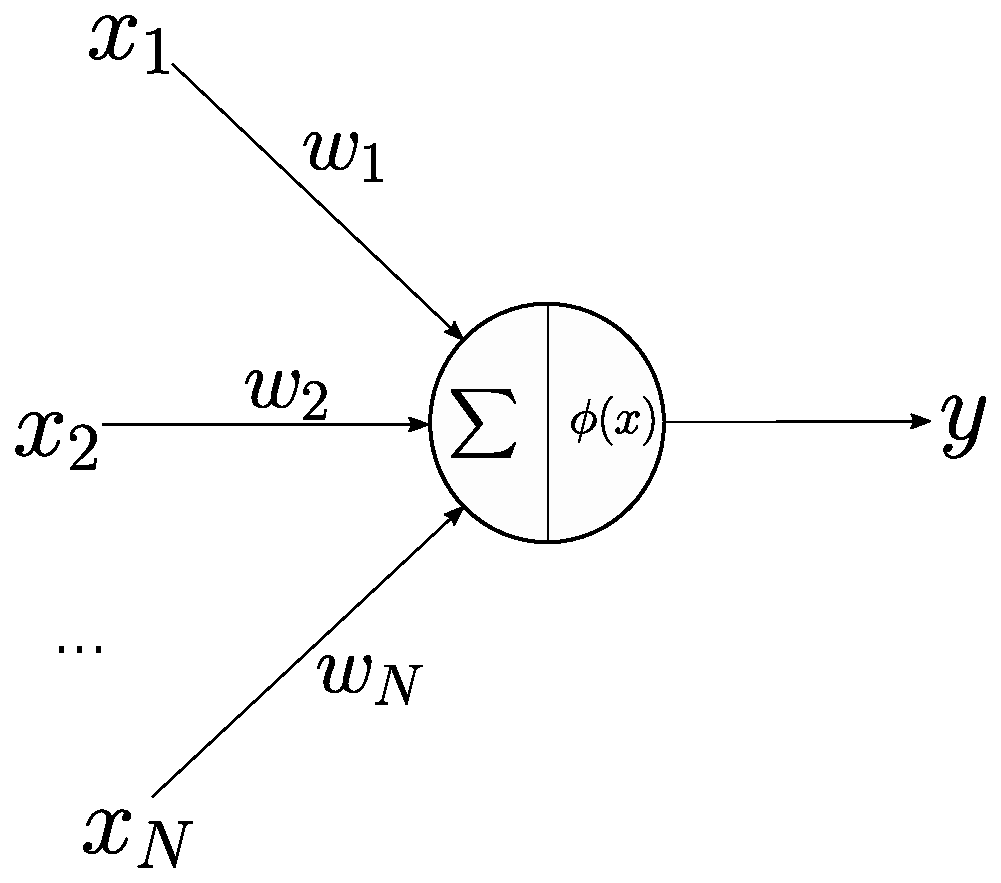
\includegraphics[width=0.5\textwidth]{perceptron-2}
	\caption[Schematischer Aufbau eines Perzeptrons]{Aufbau eines Perzeptrons: Die Eingaben $x_i$ werden gewichtet mit $w_i$ aufsummiert und nach Anwendung der Aktivierungsfunktion $\phi$ als $y$ ausgegeben.}
	% \todo{Quelle Bild!}
	\label{fig:singleNeuron}
\end{figure}

Wie in Abbildung~\ref{fig:singleNeuron} zu sehen, haben die einzelnen Eingaben \(x_i\) jeweils eine Gewichtung \(w_i\).
Es existiert ein Schwellwert oder \textit{bias}, der normalerweise 
durch eine zusätzliche Eingabe \(x_{m+1}\) mit dem Eingabewert \(+1\) und dem dazugehörigen Gewicht \(w_{m+1}\) modelliert wird.
Den Ausgabewert \(y\) erhält man dadurch, dass man die gewichteten Eingaben aufsummiert und in die Aktivierungsfunktion \( \phi \) des Perzeptrons gibt.
Mathematisch ist die Ausgabe eines Perzeptrons somit wie folgt definiert:

\begin{equation}
	y = \phi \Big( \sum_{i= 0}^{m} w_i x_i \Big) \, .
\end{equation}

Mehr Details über verschiedene Aktivierungsfunktionen, die für solch ein Perzeptron benutzt werden können, ist in Unterabschnitt~\ref{sec:activationfuncs} zu finden.
Beim Lernen werden die Gewichte \(w_i\) so angepasst, dass die gewünschte Ausgabe für die jeweilige Eingabe erreicht wird.
Bei der Auswertung verändern sich die Gewichte nicht mehr.
% \todo{Vielleicht ein paar Sätze zum Perceptron Learning Algorithm?}
Ein einzelnes Perzeptron mit zwei Eingängen kann zur Darstellung der logischen Operatoren AND, OR und NOT genutzt werden.

% Letztendlich ist ein solches Perzeptron jedoch nur ein linearer Klassifikator und kann somit 
% zum Beispiel den XOR Operator nicht auflösen.
Ein Perzeptron ist jedoch nur ein linearer Klassifikator und kann dementsprechend nur linear separierbare Probleme, wie das Problem in Abbildung~\ref{subfig:linearSep}, lösen.
Linear nicht separierbare Probleme, wie zum Beispiel der XOR-Operator oder das in Abbildung~\ref{subfig:nonlinearSep} gezeigte Problem, können nicht korrekt abbildet werden.
Dies zeigten Marvin Minksy und Seymour Papert 1969 in ihrem einflussreichen Buch \textit{Perceptrons: an introduction to computational geometry}. \todo{quelle}
% \todo[inline]{(1) lineare Trennung mit perzeptron (2) xor-problem (3) nichtlineare trennung mit dem mehrschichtigen netz}
Solche nicht linear separierbare Probleme können jedoch gelöst werden, wenn mehrere Perzeptrons hintereinandergeschaltet werden.


\begin{figure}[h]
	\centering
	\begin{subfigure}[t]{0.4\textwidth}
		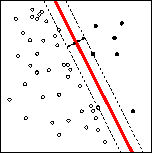
\includegraphics[width=\textwidth]{linearSep.pdf}
		\caption{Lineare Lösung für ein linear separierbares Problem.}
		\label{subfig:linearSep}
	\end{subfigure}
	\quad
	\begin{subfigure}[t]{0.4\textwidth}
		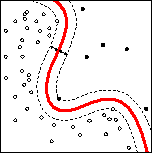
\includegraphics[width=\textwidth]{nonlinearSep.pdf}
		\caption{Nichtlineare Lösung für ein nicht linear separierbares Problem.}
		\label{subfig:nonlinearSep}
	\end{subfigure}
	\caption{Vergleich zwischen einem linear separierbaren und einem nicht linear separierbaren Problem. Angepasst von \cite{LinSep}}
	\label{fig:linearNonlinearVgl}
\end{figure}

\subsection{Feedforward Netze}

% \textbf{absatz über Feedforward Netze. Basic}
% \color{blue}
% \begin{itemize}
% 	\item Definition (keine Kreise oder Schleifen). (Kommentar Florian: \"Rückkopplung\")
% 	\item Gegenstück zum RNN
% 	\item grundlegende Architektur in Layers 
% 	\item Aktivierungsfunktionen in Layers
% 	\item Outputlayer: Verschiedene Aktivierungsfunktionen:
% 	\item Linear für regression, z.B. Softmax für Wahrscheinlichkeitsverteilung Softmax
% \end{itemize}
% \color{black}

Um die Limitation auf lineare Klassifikation eines einzelnen Perzeptrons zu überwinden, können mehrere solche Perzeptrons hintereinandergeschaltet werden. 
Die einfachste Möglichkeit dies zu tun wird als Feedforward Netz bezeichnet.
Mit diesem Begriff beschreibt man ein neuronales Netz, zwischen dessen Knoten keine Kreise beziehungsweise Schleifen existieren.
Die Informationen wandern in der Verarbeitungsrichtung von den Eingabeneuronen zu den Ausgabeneuronen.
Für gewöhnlich sind die einzelnen Knoten in Schichten, sogenannten Layers, organisiert.
Auf ein Eingabe- oder auch Input Layer folgen eine Menge an sogenannten Hidden Layers.
Den Abschluss bildet das Ausgabe- oder auch Output Layer.
Die Neuronen eines einzelnen Hidden Layers sind meist uniform und verwenden identische Aktivierungsfunktionen, wie sie in Abschnitt~\ref{sec:activationfuncs} beschrieben sind.

Je nachdem, welche Aufgabe das neuronale Netz erfüllen soll, können unterschiedliche Aktivierungsfunktionen für das Output Layer Sinn ergeben.
Häufig genutzt ist die \textit{Softmax}-Funktion für Klassifikation, da sie eine Wahrscheinlichkeitsverteilung als Ausgabe hat.
Für Regression benutzt man lineare Aktivierungsfunktionen für das Output Layer. 
Durch das Hintereinanderschalten von mehreren Layers von Neuronen mit nichtlinearen Aktivierungsfunktionen können auch Probleme, die nicht linear-separierbar sind, gelöst werden.
Tatsächlich sind solche neuronalen Netze bewiesenermaßen universale Funktionsapproximatoren -- 
sie können mit endlich vielen Neuronen in den Hidden Layers beliebige kontinuierliche Funktionen auf kompakten Subsets von \(\mathbb{R}^n\) approximieren.
Das heißt zwar, dass es theoretisch für jede solche Funktion ein Netz gibt, das sie beschreiben kann, in der Praxis muss man dieses Netz aber finden und dann auch trainieren können.
% \todo[inline]{mit Quelle belegen? Universal approximation theorem }

Es gibt viele verschiedene Unterkategorien von Feedforward Netzen, die in verschiedensten Bereichen Verwendung finden.
Convolutional Neural Networks zeichnen sich durch eine spezielle Struktur aus sogenannten Convolutional Layers aus, die als Feature Extractor fungieren.
Diese Art von Netz findet unter anderem in der Bildverarbeitung Anwendung.
Ein Netz, in dem Kreise beziehungsweise Schleifen existieren, bezeichnet man als \textit{Rekurrentes Neuronales Netz}.
Diese Netze werden vor allem dann eingesetzt, wenn die zeitliche Abfolge der Eingaben relevant ist, 
da sie im Gegensatz zu Feedforward Netzen einen internen Zustand halten.

\subsection{Aktivierungsfunktionen}
\label{sec:activationfuncs}
% \todo[inline]{Entscheiden, ob diese Section weg soll, oder auf nur ReLU reduziert werden sollte}
Es gibt verschiedene Aktivierungsfunktionen, die für den Einsatz in neuronalen Netzen in Frage kommen.
Sie sind notwendig, da ohne eine Nicht-Linearität das Netz in eine lineare Regression kollabiert, 
die dann wiederum nicht in der Lage ist nicht-lineare Funktionen darzustellen.
Sowohl die Aktivierungsfunktion als auch ihre Ableitung sollte schnell zu berechnen sein, 
da dies im Rahmen des Trainings mit dem Backpropagation Algorithmus häufig geschieht 
und sonst beträchtlicher Rechenaufwand entsteht.
% \todo[inline]{das referenziert dinge von Backprop, die der Leser hier vielleicht noch gar nicht weiß - Nach hinten?}

In der Vergangenheit wurden einige verschiedene Aktivierungsfunktionen verwendet.
% Einige häufig verwendete Aktivierungsfunktionen sollen hier vorgestellt werden.
Jede dieser Funktionen stellt eine Nicht-Linearität dar und nimmt eine einzelne Zahl, wendet eine bestimmte, festgelegte mathematische 
Operation auf diese an und gibt das Ergebnis zurück.
Historisch ist häufig die Sigmoid-Funktion \(\sigma(x)\) verwendet worden, da sie das Verhalten eines natürlichen Neurons gut nachbildet.
\begin{equation}
	\sigma(x) = \frac{1}{1 + e^x} = \frac{e^x}{e^{x + 1}}
	\label{func:Sigmoid}
\end{equation}
In der Praxis jedoch haben sich einige Nachteile der Sigmoid-Funktion und artverwandter Funktionen  gezeigt.
% \todo{Probleme mit Sigmoid genauer beschreiben? saturation}
Das schwerwiegendste davon ist die sogenannte Saturierung,
dass die Ableitung der Sigmoid-Funktion für betragsmäßig große Eingaben beinahe \(0\) ist.
Das sorgt für einen langsamen Lernprozess.
% Einige dieser Probleme konnten mit der Verwendung des Tangens hyperbolicus (tanh) behoben werden, 
% aber das Problem der Saturierung, dass ihre Ableitung bei großen Beträgen beinah \(0\) wird, nicht.
In letzter Zeit haben sich sogenannte \textit{Rectified Linear Units}, oder kurz ReLUs, durchgesetzt.
Diese sind folgendermaßen definiert:
% 
% \begin{description}
	
	% hier Könnte man die Absätze zu Sigmoid und TanH einfügen
	% \item[Sigmoid-Funktion] \hfill \\
		\begin{equation}
			f(x) = \frac{1}{1 + e^x} = \frac{e^x}{e^{x + 1}}
			\label{func:Sigmoid}
		\end{equation}
		\begin{equation}
			f'(x) = f(x) * (1 - f(x))
		\end{equation}
		Die mathematische Form der Sigmoid Aktivierungsfunktion ist in Abbildung \ref{sigmoidFunc} zu sehen.
		Sie bildet die reellen Zahlen \(\mathbb{R}\) auf das Intervall \((0,1)\) ab. 
		Für betragsmäßig größer werdende negative Zahlen nähert sich der Rückgabewert \(0\) an,
		ebenso wie für größer werdende positive Zahlen sich der Rückgabewert an \(1\) annähert.

		Die Sigmoid Funktion ist eine historisch häufig genutze Funktion, da sie das Verhalten eines natürlichen Neurons,
		der biologischen Motivation für künstliche Neuronen, gut nachbildet:
		komplette Inaktivität eines Neurons bei Ausgabe 0 bis zum feuern mit maximaler Frequenz bei Ausgabe 1.

		In der Praxis jedoch haben sich einige Nachteile der Sigmoid Funktion gezeigt, weshalb sie quasi nicht mehr genutzt wird.
		Der gewichtigste von diesen ist, dass ihre Ableitung bei großen Beträgen beinah \(0\) ist.
		Dies führt dazu, dass während der Ausführung des Backpropagation-Algorithmus beinah keine Änderungen passieren und dementsprechend das Netz sehr langsam lernt.
		
		\begin{figure}
			\centering
			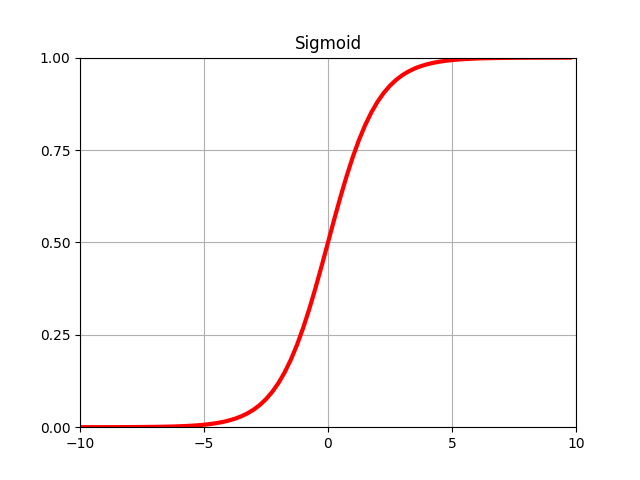
\includegraphics[width=0.618\textwidth]{Sigmoid}
			\caption{Plot der Sigmoid Funktion}
			\label{sigmoidFunc}
		\end{figure}
		  


	\item[TanH] \hfill \\
		\begin{equation}
			f(x) = \tanh(x) = \frac{e^x - e^{-x}}{e^x + e^{-x}}
		\end{equation}
		\begin{equation}
			f'(x) = 1 - f(x)^2
		\end{equation}
		Die TanH-Aktivierungsfunktion ist in Abbildung \ref{tanhfunction} dargestellt.
		Im Gegensatz zur Sigmoid Funktion bildet sie die reellen Zahlen \(\mathbb{R}\) auf das Intervall \((-1, 1)\) ab.
		Weil sie zentriert um den Nullpunkt ist, wird sie bei realen Anwendungen der Sigmoid Funktion vorgezogen.
		Das Saturationsproblem der Sigmoid Funktion besteht jedoch immer noch.
		\begin{figure}
			\centering
			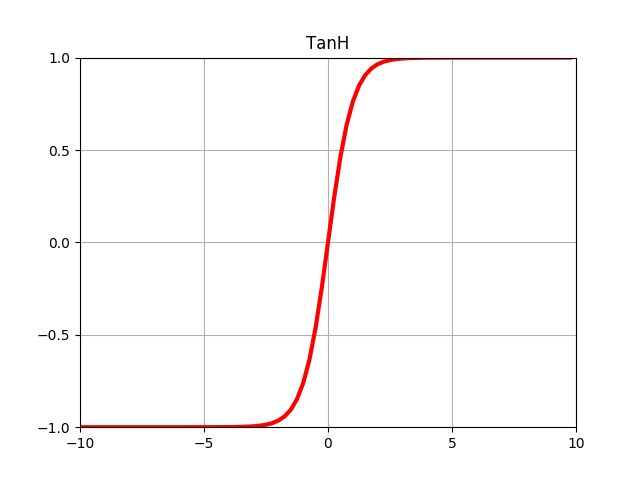
\includegraphics[width=0.618\textwidth]{Tanh}
			\caption{Plot der Tanh Funktion}
			\label{tanhfunction}
		\end{figure}
	
	% \item[ReLU] \hfill \\
\begin{equation}
	f(x) = \max(0, x) \, ,
\end{equation}
\begin{equation*}
	f'(x) = \begin{cases}
	0 &\text{, falls $x < 0$}\\
	1 &\text{, falls $x > 0$}
	\end{cases} \, .
\end{equation*}
\todo[inline]{sicherstellen dass das nicht so über die seite umgebrochen wird}

\begin{figure}[h]
	\centering
	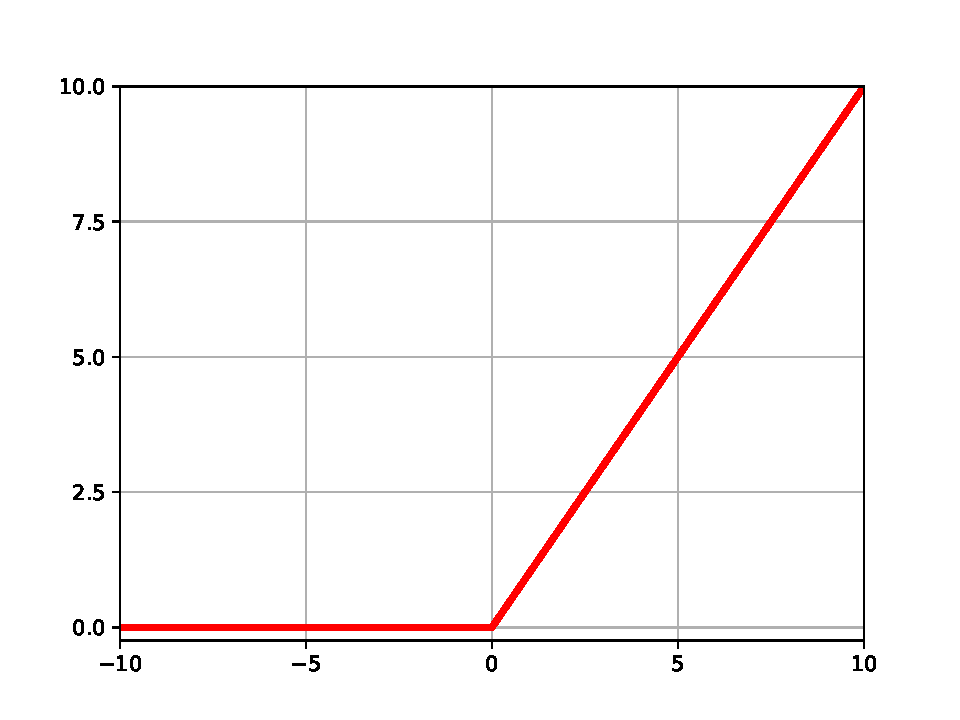
\includegraphics[width=0.618\textwidth]{reluPlot.pdf}
	\caption{Schaubild der Ausgabe einer ReLU.}
	\label{reluoutput}
\end{figure}
Abbildung~\ref{reluoutput} zeigt das Schaubild einer solchen ReLU. 
% \todo{ReLU plot neu machen: dicker bei unter 0 und als Vector graphic statt als PNG}
Die Aktivierung von ReLUs ist ein einfacher Schwellwert, der weit weniger rechenintensiv ist als die aufwendigen Exponentialfunktionen von Sigmoid und tanh.
In der Praxis hat sich zudem gezeigt, dass ReLUs oft deutlich schneller konvergieren als Sigmoid- oder tanh-Neuronen, da sie kein Problem mit Saturierung haben.
Krizhevsky et al. haben in ihrem Paper~\cite{NIPS2012_4824} einen Geschwindigkeitsgewinn um Faktor 6 feststellen können.

Ein Problem, das mit ReLUs jedoch existiert ist, dass einzelne Neuronen während dem Training "absterben" können, falls sie irgendwann in dem Bereich landen, in dem der Gradient 0 ist.
Diese Neuronen sind dann für jeden beliebigen Input inaktiv und können niemals wieder etwas zur Ausgabe des Netzes beitragen.
Durch die Wahl einer geeigneten Lernrate oder den Einsatz sogenannter Leaky ReLUs lässt sich dies jedoch vermeiden.
Leaky ReLUs haben im Gegensatz zu normalen ReLUs eine kleine positive Steigung im negativen Bereich.
\begin{equation}
	f(x) = \begin{cases}
		x &\text{, falls } x  >  0\\
		0.01 x &\text{, falls } x  \leq  0
	\end{cases}
\end{equation} 






% \end{description}

% \begin{figure}[h]
%     \centering
%     \begin{subfigure}[t]{0.3\textwidth}
% 		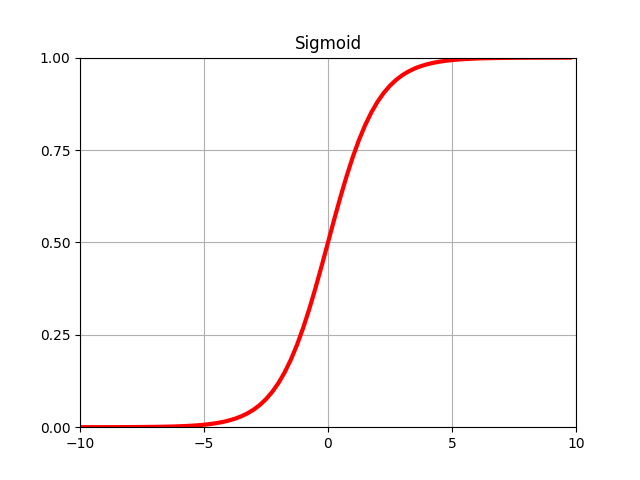
\includegraphics[width=\textwidth]{Sigmoid}
% 		\caption{Sigmoid Funktion}
%     \end{subfigure}
%     \begin{subfigure}[t]{0.3\textwidth}
% 		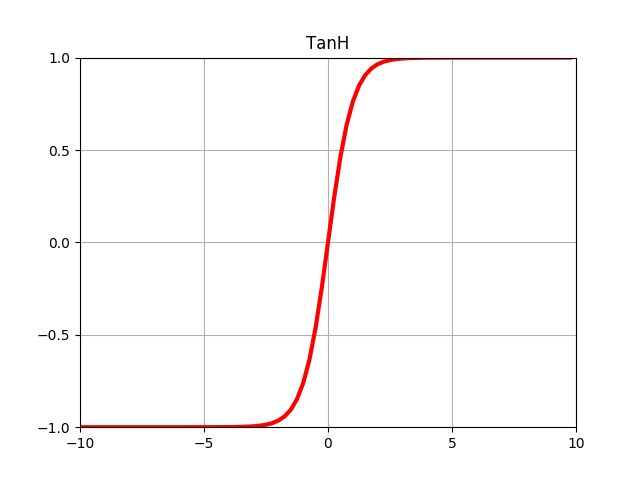
\includegraphics[width=\textwidth]{Tanh}
% 		\caption{TanH Funktion}
%     \end{subfigure}
%     \begin{subfigure}[t]{0.3\textwidth}
%         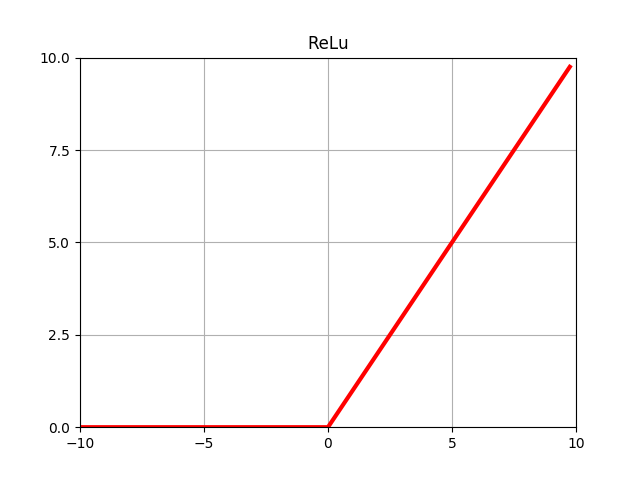
\includegraphics[width=\textwidth]{ReLu}
%         \caption{ReLU}
%     \end{subfigure}
%     \caption{Häufig verwendete Aktivierungsfunktionen}
%     \label{eval:function}
% \end{figure}





% \subsection{Backpropagation}

% \todo[inline]{Optional: am Ende entscheiden ob ich noch mehr Kontent möchte und dann gegebenenfalls ausformulieren}
% Der Backpropagation Algorithmus ist ein Verfahren, mit denen künstliche neuronale Netze in der Lage sind, komplizierte Zielfunktionen einzulernen.
% Es ist eine Methode, bei der effizient der Gradient der Fehlerfunktion in Abhängigkeit vom Gewicht der einzelnen Kanten im Netz bestimmt werden kann,
% was dann für einen Gradientenabstieg verwendet werden kann. 

% \color{blue}
% \begin{itemize}
% 	\item Definition und Beschreibung
% 	\item Nur supervised learning: Gradient der Fehlerfunktion wird benötigt \(\rightarrow\) Tatsächliches Ergebnis muss bekannt sein.
% 	\item "Finden einer Funktion, die am besten die Inputs auf die outputs mapt"
% \end{itemize}
% \color{black}

\subsection{Performance-Maß}

Neuronale Netze werden in der Regel danach bewertet, wie gut sie mit unbekannten, das heißt nicht im Training vorgekommenen, Daten umgehen können.
% Das essenzielle Maß nachdenen neuronale Netze bewertet werden, ist wie gut sie mit neuen, unbekannten Daten umgehen, die nicht in den Trainingsdaten vorhanden waren. 
Diese Eigenschaft von Trainingsdaten auf unabhängige Testdaten schließen zu können wird Generalisierung genannt. 

Als Overfitting bezeichnet man es, wenn ein gelerntes Modell sich zu sehr an den zum gegebenen Training betrachteten Datensatz anpasst und 
dafür in Kauf nimmt, zusätzliche oder zukünftige Daten schlechter zu repräsentieren.
Das Modell wird also schlechter darin zu generalisieren.
Speziell im Feld der neuronalen Netze ist Overfitting meist daran zu erkennen,
dass sich die Qualität der Ausgaben des Netzes auf dem Trainingsdatenset weiter verbessert,
während sie auf dem Testdatenset schlechter wird.
Dies kann zum Beispiel der Fall sein, wenn das Modell Rauschen in den Trainingsdaten als Teil der zugrundeliegenden Struktur interpretiert. 


Dem Overfitting gegenüber steht das Underfitting. 
Als Underfitting bezeichnet man wenn das Netz nicht in der Lage ist
eine ausreichend gute Performance auf den Trainingsdaten zu erreichen.
Das kann passieren, wenn das Modell nicht ausreichend komplex ist, um die zugrundeliegende Struktur der Daten abzubilden.
Sowohl Overfitting als auch Underfitting hängen mit der Kapazität eines Netzes zusammen.
Ist die Kapazität zu gering, kann es sein, dass das Netz daran scheitert die Trainingsdaten zu lernen.
Ist die Kapazität zu groß, so kann es passieren, dass das Netz gewissermaßen die Trainingsdaten einfach auswendig lernt.
% \todo{umgangsprachlich mit einer besseren Formulierung ersetzen...}
Dies ist beispielhaft in Abbildung~\ref{fig:capacity} zu sehen.
Aus der zugrundeliegenden Cosinus Funktion werden Stichproben mit einem Rauschterm entnommen. 
Stellvertretend für das Lernen mit neuronalen Netzen wird hier lineare Regression benutzt,
um die Parameter eines Polynoms zu lernen.
Die Kapazität des Modells wird hier durch den Grad des Polynoms festgelegt.

In Abbildung~\ref{subfig:underfitting} wird ein Polynom mit dem Grad 1 gelernt.
Die Kapazität ist zu niedrig und dementsprechend schafft das Modell es nicht die Stichproben akkurat zu repräsentieren.
In Abbildung~\ref{subfig:rightfitting} ist der Grad des Polynoms 4.
Das resultierende Modell ist eine gute Approximation der ursprünglichen Funktion.
In Abbildung~\ref{subfig:overfitting} ist der Grad des Polynoms mit 17 deutlich zu hoch.
Man kann am resultierenden Modell erkennen, wie es dem Rauschen der Samples folgt und wie es an den Rändern des betrachteten Bereichs schnell divergiert.

Die beste Methode, um Overfitting zu vermeiden, ist es, mehr Trainingsdaten zu benutzen.
In der Praxis kann dies oft umständlich, kostspielig oder sogar unmöglich sein, 
weshalb auf das Generieren von synthetischen Trainingsdaten, auch Datenaugmentierung genannt, zurückgegriffen wird.
% There is no Data like more Data
Auch der Einsatz von Regularisierungsverfahren kann helfen Overfitting zu verringern.
Als letzter Schritt kann die Kapazität der Architektur gesenkt werden,
zum Beispiel, indem die Anzahl der zur Verfügung stehenden Layer reduziert wird.


% \color{blue}
% \begin{itemize}
% 	\item Methoden um Overfitting zu vermeiden:
% 	\item Mehr Trainingsdaten (z.\,B. durch Data-Augmentation)
% 	\item Regularisierung (L1, \(L_2\) (siehe unten), dropout)
% \end{itemize}
% \color{black}

\subsection{Regularisierung} \label{ssec:Regul}

% \color{blue}
% \begin{itemize}
% 	\item Regularisierung Definition
% 	\item Mathematische Formel Darstellung
% 	\item \(L_1\) und \(L_2\) Regularisierung
% 	\item L0 - warum nicht?
% 	\item (Maybe Dropout)
% 	\item Early Stopping? (das internet sagt, es ist eine art von Regularisierung und falls ich sie verwenden sollte, sollte ich sie hier erwähnen)
% \end{itemize}
% \color{black}

Als Regularisierung bezeichnet man Techniken, die zur Vermeidung von Overfitting verwendet werden.
% Sie wird in der Hoffnung angewendet, dass das Modell mit Regularisierung besser generalisiert als ohne.
Viele Techniken des maschinellen Lernens funktionieren so, dass sie den Fehler auf den Trainingsdaten reduzieren und damit potenziell indirekt auch den auf den Testdaten.
Im Gegensatz dazu soll hier primär der Fehler auf den Testdaten reduziert werden, selbst wenn das zu schlechteren Ergebnissen auf den Trainingsdaten führt.
Das Ziel ist also bessere Generalisierung.

Eine Möglichkeit ist, dass zur Loss-Funktion ein Regularisierungsterm \(R\) hinzugefügt wird, 
der die Kosten basierend auf der Komplexität des Systems erhöht.
 
\begin{equation}
	\min_f \sum\limits_{i=1}^{m} V(f(\vec{x}_i), \vec{y}_i) + \lambda R(f)
\end{equation} 
 
Dabei ist \(V\) die Loss-Funktion, beispielsweise \textit{Mean-Square-Error} oder \textit{Mean-Absolute-Error}.
\(m\) ist die Anzahl der Feature-Label-Paare,
\(x_i\) und \(y_i\) sind die einzelnen Eingabefeatures und das dazugehörige Label.
Die Funktion \(f\) ist in unserem Fall das neuronale Netz, das die Features entgegennimmt.
\(\lambda\) ist ein Parameter, der die Gewichtung des Regularisierungsterm festlegt.
Wählt man diesen Parameter zu klein, so kann es sein, dass das Modell trotz Regularisierung noch immer overfittet.
Wählt man ihn zu groß, so kann es sein, dass das Modell das Problem nicht mehr korrekt abbildet und es zu Underfitting kommt.
Der Regularisierungsterm \(R\) wird so gewählt, dass er die Komplexität der Funktion \(f\) widerspiegelt.
Ein gutes Maß für die Komplexität eines neuronalen Netzes sind die Gewichte zwischen den Neuronen.
Beispiele für \(R\) wären zum Beispiel die \(L_1\)- oder die \(L_2\)-Regularisierung. % die jeweils mit der \(L_1\) beziehungsweise mit der \(L_2\)-Norm arbeiten.
Der entscheidende Unterschied zwischen den beiden ist ein unterschiedlicher Strafterm, zu sehen in Gleichung~\eqref{eq:MSE-L1} für \(L_1\) und Gleichung~\eqref{eq:MSE-L2} für \(L_2\). 
Die Fehlerfunktionen sind jeweils MSE mit dazugehörigen Strafterm.

\begin{equation} \label{eq:MSE-L1}
	J(X, Y) = \frac{1}{m} \sum_{i=1}^{m} (\vec{y}^{(i)} - \hat{\vec{y}}^{(i)})^2 + \sum_{j, k} (|\mat{W}_{j,k}|)
\end{equation} 

\begin{equation} \label{eq:MSE-L2}
	J(X, Y) = \frac{1}{m} \sum_{i=1}^{m} (\vec{y}^{(i)} - \hat{\vec{y}}^{(i)})^2 + \sum_{j, k} (\mat{W}_{j,k}^2)
\end{equation} 


Ein Regressionsmodell, das \(L_1\)-Regularisierung verwendet, wird auch als Lasso Regression bezeichnet, 
während ein Modell mit \(L_2\)-Regularisierung als Ridge Regression beschrieben werden kann.
Vergleicht man die beiden Ansätze, so schrumpft die \(L_1\)-Norm weniger wichtige Gewichte auf 0, was zu dünn besetzten Gewichtsvektoren führt.
Dies kann eine wünschenswerte Eigenschaft sein.
Im Gegensatz dazu hat die \(L_2\)-Regularisierung den Vorteil, dass sie effizienter berechnen kann.
Der Strafterm von \(L_2\) hat eine geschlossene Form und kann in Form einer Matrix angewendet werden, während die Funktion von \(L_1\) auf Grund des Betrags eine nicht-differenzierbare ist.


% \todo{absatz zu (L0 und warum man es nicht benutzt?)}

Eine weitere Regularisierungstechnik ist Dropout~\cite{JMLR:v15:srivastava14a}.
Dabei werden während dem Training eines neuronalen Netzes 
mit einer festgelegten Wahrscheinlichkeit zufällig Neuronen und die dazugehörigen Verbindungen abgeschaltet, 
wie in Abbildung~\ref{fig:dropout} dargestellt.
% \todo{Ist die Grafik essenziell fürs Verständnis?}
Dies soll insofern Overfitting vermeiden, dass es übermäßige Koadaption von mehreren Neuronen erschwert.
Dropout als Technik wird insbesondere bei tiefen neuronalen Netzen mit einer hohen Anzahl von Hidden Layers eingesetzt. 
Als Early Stopping wird eine Technik bezeichnet, bei der die Regularisierung durch das frühzeitige Beenden des Trainings erreicht wird \cite[Kapitel 7.8]{Goodfellow-et-al-2016}.
Dabei wird versucht abzuschätzen, an welchem Punkt des Trainings 
eine Verbesserung der Ergebnisse auf dem Trainingsset zu Lasten der Ergebnisse auf dem Testset geschieht.


\begin{figure}
    \centering
    \begin{subfigure}[t]{0.4\textwidth}
		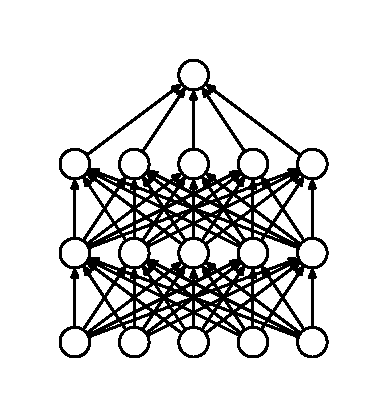
\includegraphics[width=\textwidth]{neuralNet}
		\caption{Unverändertes neuronales Netz}
    \end{subfigure}
    \begin{subfigure}[t]{0.4\textwidth}
		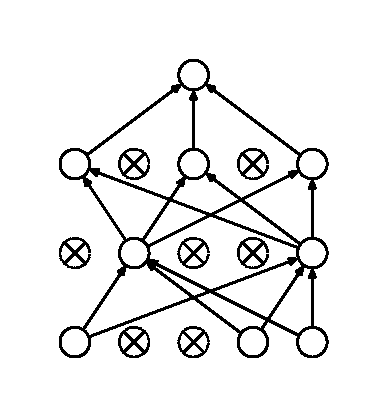
\includegraphics[width=\textwidth]{neuralNet_dropped}
		\caption{Nach Dropout Anwendungen.}
	\end{subfigure}
    \caption{Beispiel für die Dropout-Regularisierung~\cite{JMLR:v15:srivastava14a}.}
    \label{fig:dropout}
\end{figure}


\begin{figure}
    \centering
	
	\begin{subfigure}[t]{0.6\textwidth}
		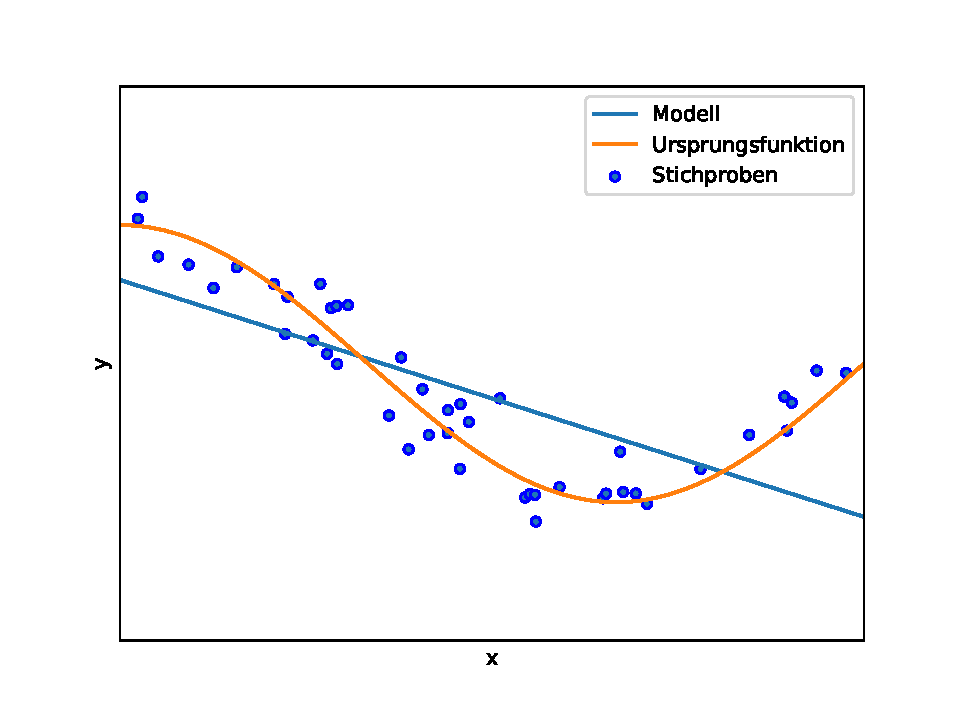
\includegraphics[width=\textwidth]{plotUnderfitting.pdf}
		\caption{Underfitting mit Polynom von Grad 1}
		\label{subfig:underfitting}
	\end{subfigure}
	% \quad
	\begin{subfigure}[t]{0.6\textwidth}
		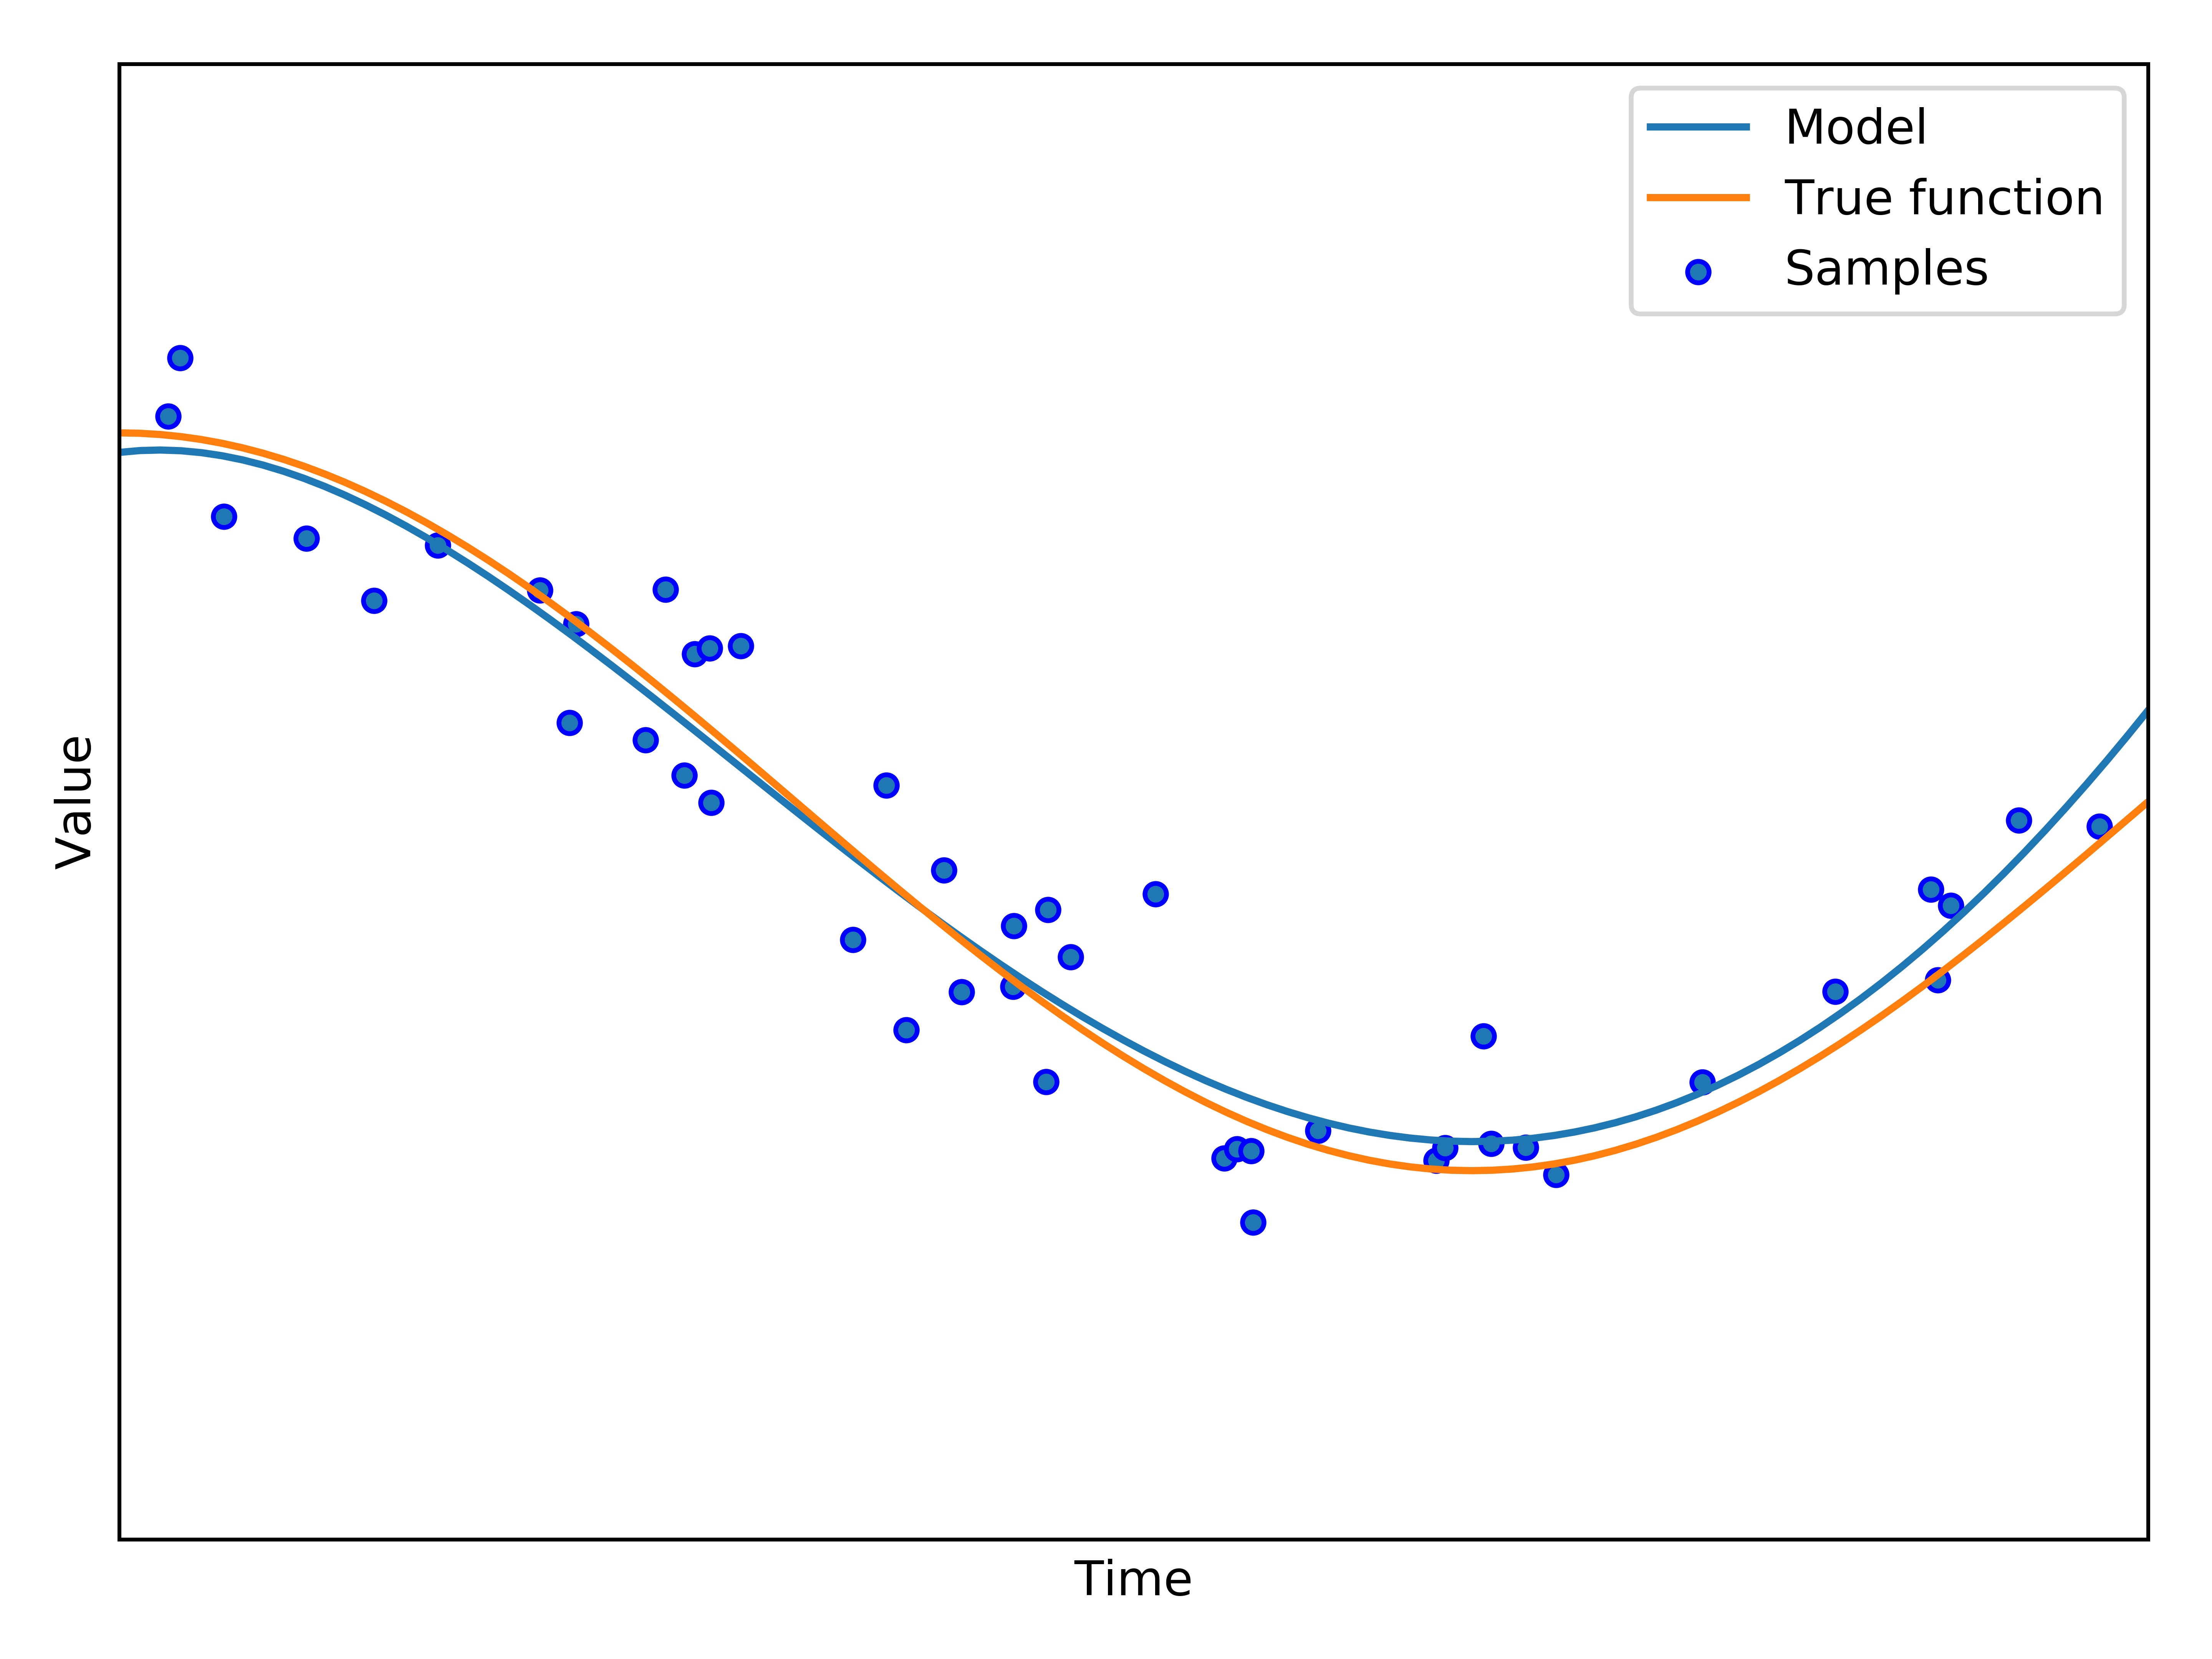
\includegraphics[width=\textwidth]{plotPassendesModell.pdf}
		\caption{Passendes Modell -- ein Polynom von Grad 4}
		\label{subfig:rightfitting}
	\end{subfigure}
	% \quad
	\begin{subfigure}[t]{0.6\textwidth}
        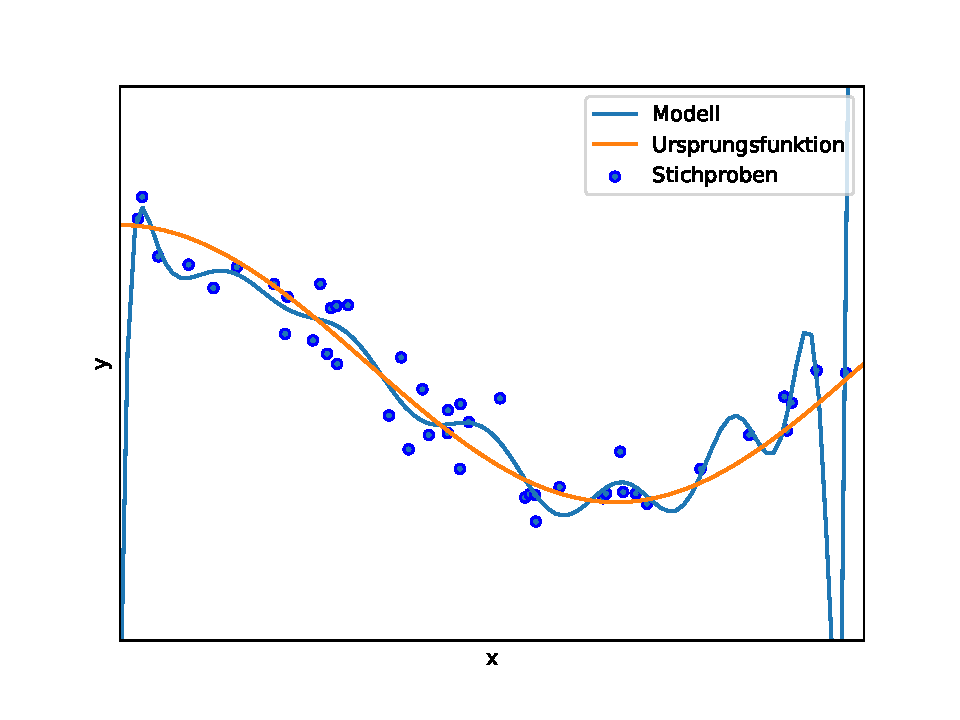
\includegraphics[width=\textwidth]{plotOverfitting.pdf}
		\caption{Overfitting mit Polynom von Grad 17}
		\label{subfig:overfitting}
	\end{subfigure}
	\caption{Visualisierung von Modellen mit unterschiedlichen Kapazitäten.}
	\label{fig:capacity}
\end{figure}


\section{TableSort System}

% \todo[inline]{Viel stuff über das TableSort System}
% \color{blue}

% \begin{itemize}
% 	\item kleiner, experimenteller Bandsortierer~\cite{doll2015}
% 	\item Entstanden in Kooperation zwischen dem Fraunhofer IOSB, Abteilung Sichtprüfsysteme, und dem Institut für Intelligente Sensor Aktor Systeme des Karlsruher Institut für Technologie.
% 	\item Im Rahmen des \textit{TrackSort} Projekts
% 	\item Gedacht für Experimente, wenn es zu aufwendig ist das mit dem großen großen zu machen und zum Mitnehmen auf Messen.
% 	\item 2 Modi: mit Förderband und mit Rutsche
% 	\item Mit Flächenkamera für TrackSort als auch die Zeilenkamera sind dargestellt.
% 	\item Ringlicht (Refence später)
% 	\item Die Zeilenkamera wird zurzeit in industriellen Schüttgutsortieranlagen verwendet, ist aber nicht optimal (Siehe all die Literatur)
% \end{itemize}
% \color{black}


Der \textit{TableSort}-Schüttgutsortierer ist eine modulare Versuchsplattform, die konzipiert wurde, um neue Schüttgutsortierkonzepte in einem kleineren Rahmen experimentell erproben zu können.
Industrielle Schüttgutsortieranlagen sind sehr groß und um etwas an ihrer Konfiguration zu ändern ist sowohl zeitaufwendig als auch arbeitsintensiv.
Daher ist es sinnvoll eine Plattform zu haben, die flexibel und transportabel ist und leicht umgebaut werden kann.
Das System ist im Rahmen des \textit{TrackSort} Projekts in Kooperation zwischen dem Fraunhofer IOSB, Abteilung Sichtprüfsysteme, und dem Institut für Intelligente Sensor Aktor Systeme des Karlsruher Institut für Technologie entstanden\cite{doll2015}.
Es kann in zwei verschiedenen Transportkonfigurationen benutzt werden.
Einmal werden die Schüttgutpartikel mittels eines Förderbands beschleunigt.
Diese Konfiguration ist in Abbildung~\ref{fig:tablesortsystem} zu sehen.
Dazu kommt die Möglichkeit das Förderband mit einer Rutsche zu ersetzen, sodass die Schüttgutpartikel stattdessen durch die Schwerkraft beschleunigt werden. 
Im Rahmen dieser Arbeit wurde die Flächenkamera-Konfiguration mit einem Ringlicht zur Beleuchtung verwendet.
Schematisch ist der Ablauf der Schüttgutsortierung in Abbildung~\ref{fig:aufbau_tablesort} zu sehen.
Die Funktionsweise des Systems wird im Folgenden erklärt.
Das zu sortierende Schüttgut wird durch einen Schwingförderer nach und nach über eine Rutsche auf das Förderband aufgebracht.
Dort wird es in Richtung des Druckluftdüsenarrays beschleunigt. 
Auf das vom Ringlicht beleuchtete Ende des Förderbands ist die Flächenkamera gerichtet.
Kurz nachdem die Schüttgutpartikel die Flugphase beginnen, passieren sie das Druckluftdüsenarray.
Dort werden sie abgelenkt, falls die Verarbeitung der Bilddaten von der Kamera sie als auszusortieren klassifiziert.

\begin{figure}[h]
	% \missingfigure{Bild von TablesortSystem}
	\includegraphics[width=\textwidth]{TrackSortPic}
	\caption{TableSort Schüttgutsortiersystem \cite{fraunhoferiosb2017}}
	% \todo{Quelle Bild!}
	\label{fig:tablesortsystem}
\end{figure}


\begin{figure}[h]
    \centering
    \def\svgwidth{\columnwidth}
	\input{img/Aufbau-moved.pdf_tex}
	\caption[Schematische Darstellung des optischen Bandsortierers TableSort nach~\cite{Pfaff2017}.]{
		Schematische Darstellung des optischen Bandsortierers TableSort nach~\cite{Pfaff2017}.
	}
	\label{fig:aufbau_tablesort}

\end{figure}


